\documentclass[a4paper, 11pt]{article}
\usepackage[top = 1.1in, bottom = 1.1in, left = 0.6in, right = 0.6in]{geometry}
\usepackage{amsmath}
\usepackage{graphics}
\usepackage{graphicx}
\usepackage{subcaption}
\usepackage{caption}
\usepackage{listings}
\usepackage{multirow}
\usepackage{multicol}
\usepackage{url}
\usepackage[export]{adjustbox}
\usepackage[labelfont=bf]{caption}

\usepackage{lipsum}
\newenvironment{Figure}
  {\par\medskip\noindent\minipage{\linewidth}}
  {\endminipage\par\medskip}

\begin{document}
%%Title
\Large
\begin{center}
\hrulefill \\
\textbf{IMAGE PROCESSING} \\
SF2 - FINAL REPORT \\
\vspace{0.2cm}
\normalsize 
Quang-Thinh Ha - CRSid: qth20 \\
\hrulefill \\
\end{center}

\normalsize

\section{Introduction}
This is the final report for this project. The report aims at exploring further possible strategies for image compressing algorithms. The report will conclude with a finalised solution for the problem. 

Since at this state of the project involves cooperation between two individuals, this report will make references based on the conclusion made by Rajiv A. Kurien, who is the other member of the team.

\section{Centre-clipped linear quantisers}
The first approach would be to quantise more samples to zero. As the probability distributions of the intensities of the bandpass sub-images from the energy compaction are usually highly peaked at zero, it is desirable to widen the step-size of the `zero' step. 

In this report, the effect of varying the first rise of the quantiser is investigated on the LBT\footnote{Lapped-Biorthogonal Transform.} scheme. The performance observed from Figure \ref{fig:cr_rise1} indicates that a ratio of roughly 1 between \textbf{rise1} and \textbf{step} gives the highest compression ratio. 

Also, when looking at the changes in quantising error against the number of bits over different ratios between \textbf{rise1} and \textbf{step} in Figure \ref{fig:rms_bits}, the RMS error reduces with increasing number of bits for coding the image.This is as expected, as the more bits there are to code the decoded image, the more closely assemble the re-constructed image should be to the original version. RMS error, hence, reduces. 

When looking at the image quality, widening the `zero' step size does not significantly decrease the image quality. Figure \ref{fig:0.5_0.75_rise1} shows that the differences observed when widening the `zero' step size is unrecognisable, so it is encouraged to \textit{quantise more values to zero}, as this gives a higher compression ratio while maintaining good quality of the re-constructed image. 

Based on the same principle, let's look at the effect on the constructed image of DCT when some of the coefficients is compressed. Figure \ref{fig:cr_suppress} shows that, as expected, the more high-frequency components term is suppressed, the larger the compression ratio would become. The significant rise at the end is when more that $80\%$ of the high-frequency coefficients have been suppressed. However this huge increase shows significant loss in image quality. Figure \ref{fig:0.5_0.75_rise1} shows that until 49 out of 64 of the DCT coefficients is suppressed, there won't be any significant decrease on the image quality. 

\newpage
\section*{APPENDIX}
\begin{multicols}{2}
\begin{Figure}
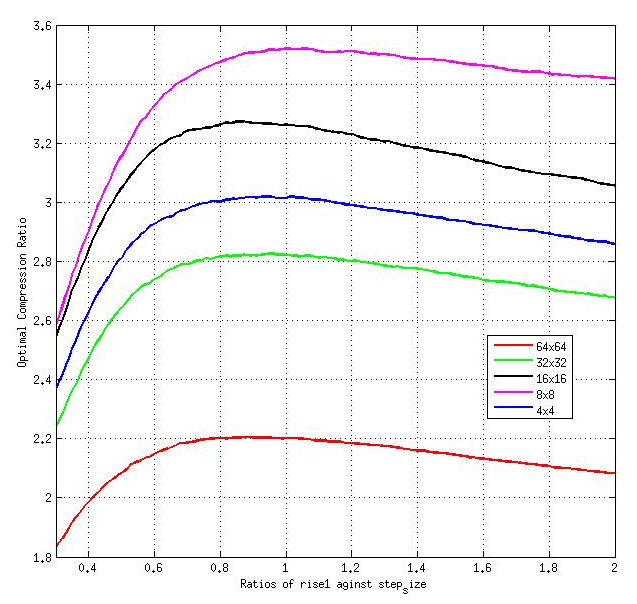
\includegraphics[width=1.0\linewidth, center]{cr_rise1.jpg}
\captionof{figure}{\small{\textbf{Effects of varying the `zero' step when quantising the image.} The x-axis represents the ratio between the `zero' step and the normal quantise steps. Larger ratio leads to wider `zero' steps, which leads to more values being quantised to 0. The colour lines indicate different transform sizes of LBT.}}
\label{fig:cr_rise1}
\end{Figure}

\begin{Figure}
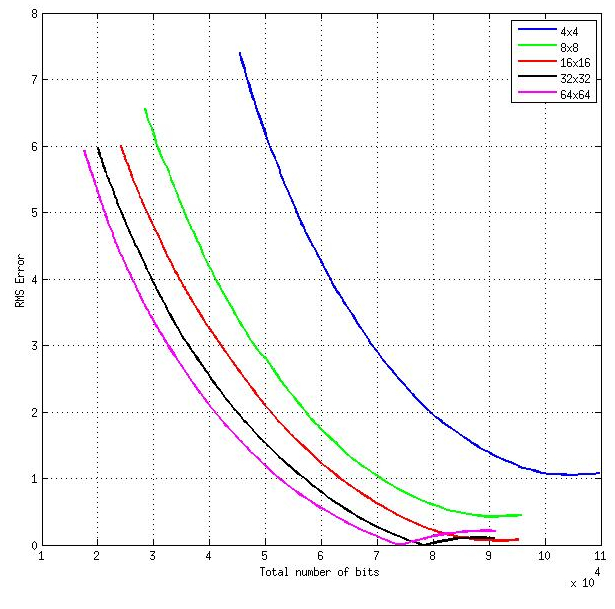
\includegraphics[width=1.0\linewidth, center]{rms_bits.jpg}
\captionof{figure}{\small{\textbf{Effects of varying the ratio between `zero' on the relationship between quantising error against the number of bits.} The RMS error is compared to the \textit{reference scheme} error, which is obtained when quantising the original image with 17 steps. Note also that the ratio is only varied from 0.3 to 2.0, which corresponds to the tailing/plateau value of these plots. }}
\label{fig:rms_bits}
\end{Figure}

\begin{Figure}
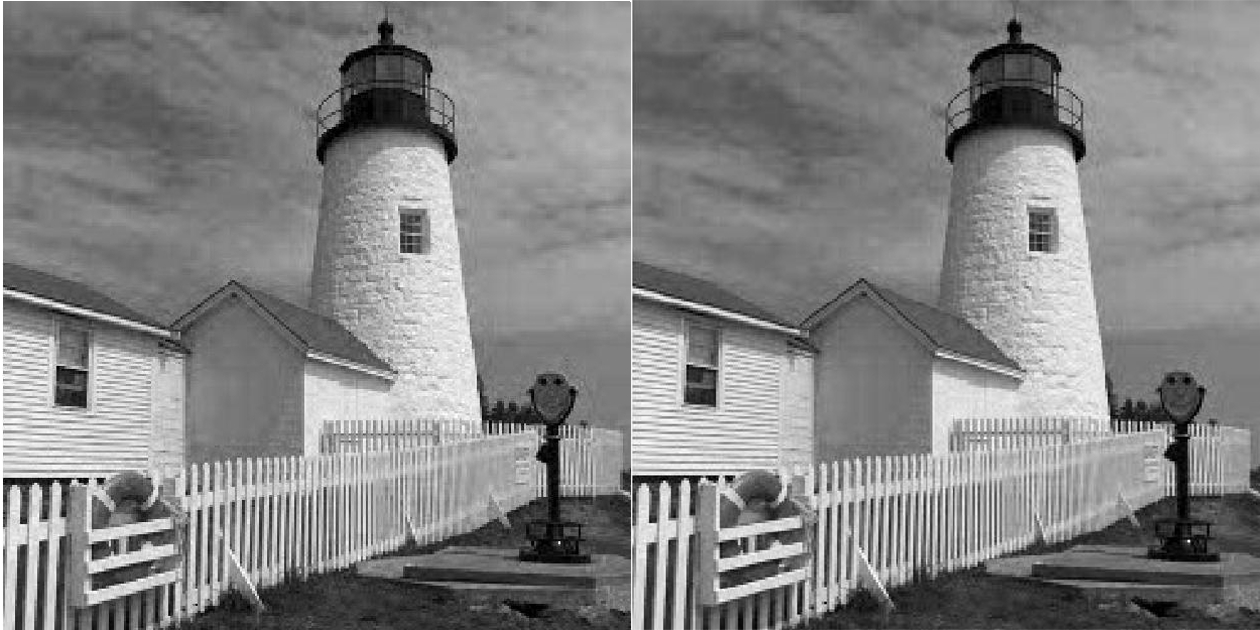
\includegraphics[width=1.0\linewidth, center]{05_075_rise1.jpg}
\captionof{figure}{\small{\textbf{Visual differences when using different width of the `zero' step.} The cloud does look a bit different between the `zero' step width of $0.5 \times step$ on the left and $0.75$ on the right. Apart from that, it is really debatable that there are huge differences between the two pictures.}}
\label{fig:0.5_0.75_rise1}
\end{Figure}

\begin{Figure}
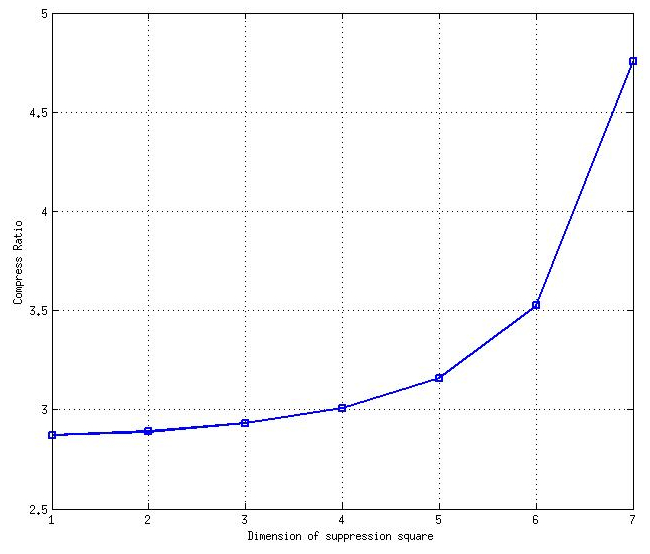
\includegraphics[width=1.0\linewidth, center]{cr_suppress.jpg}
\captionof{figure}{\small{\textbf{Increase in compress ratio when some coefficients of DCT is suppressed.} The x-axis indicates the dimension of the $n\times n$ of the decoded image that is suppressed. This is equivalent to setting $n\times n$ frequency terms to 0 when reconstructing the image.}}
\label{fig:cr_suppress}
\end{Figure}

\begin{Figure}
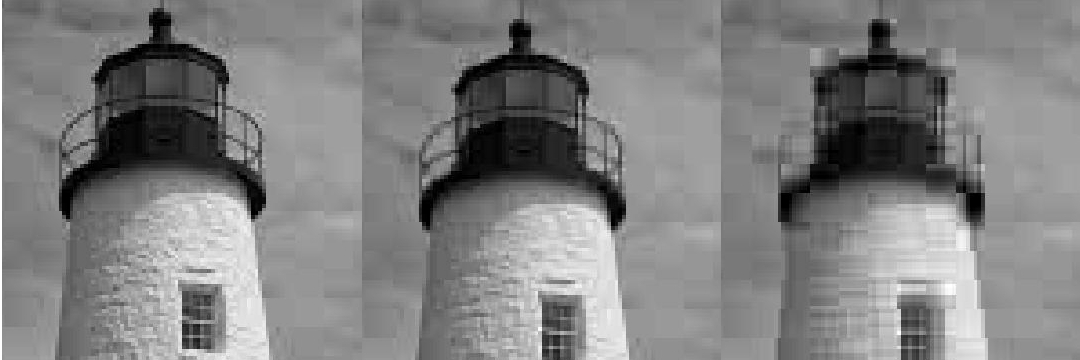
\includegraphics[width=1.0\linewidth, center]{dct_clear_3_5_7.jpg}
\captionof{figure}{\small{\textbf{Visual quality on suppressing high-frequency components.} There is no significant changes until most of the high-frequency terms have been suppressed. }}
\label{fig:dct_clear_3_5_7}
\end{Figure}

\end{multicols}{2}

\end{document}
